\renewcommand{\thesubsection}{ \Alph{subsection}}

\section*{Appendix}

\subsection{Openmarkov}\label{org.openmarkov}

\begin{center}
	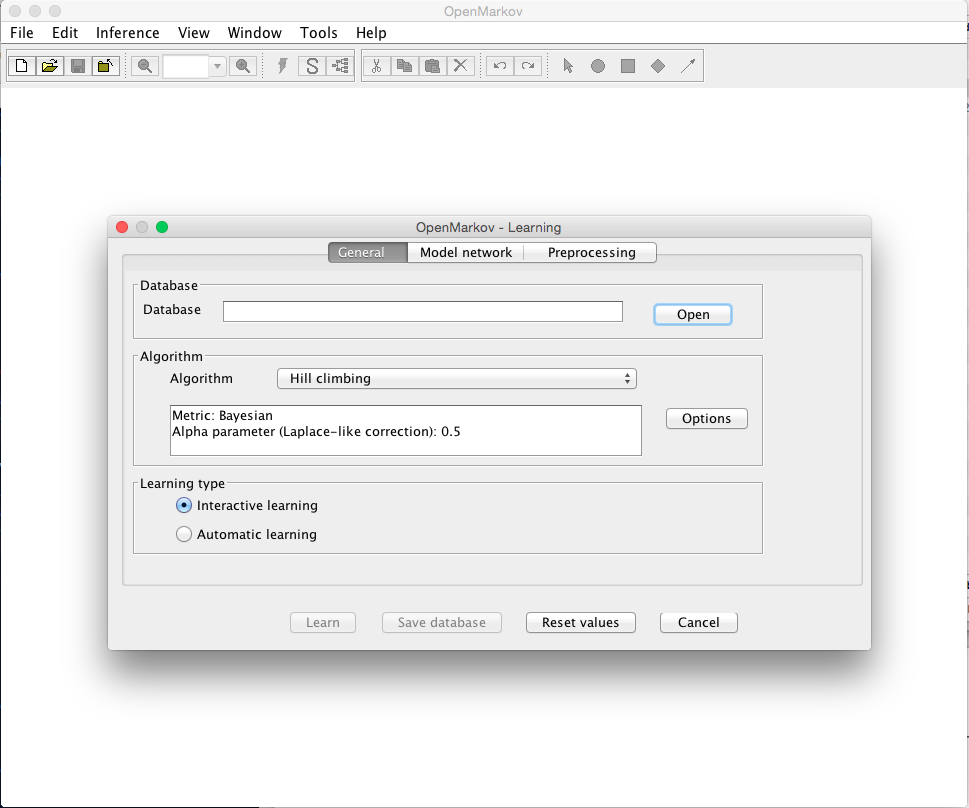
\includegraphics[width=1.00\textwidth]{content/pictures/openmarcov.png}
\end{center}
\pagebreak

\subsection{Interaktives Strukturlernen}\label{interactive}
Reihenfolge des Hinzufügens der Links.\\
 \hspace*{3mm}
 \begin{tabular}{lcr}
  \textbf{Link} & \textbf{Motivation} \\
  Mathe --> Physik & 81.03 \\
  Mathe --> OLT-Mathe & 49.20 \\
  Mathe --> Abschluss & 45.37 \\
  Schultyp --> Qualifikation & 38.63 \\
  Schultyp --> Deutsch & 38.81 \\
  Schultyp --> Mathe & 38.36 \\
  Deutsch --> OLT-Deutsch & 28.62 \\
  Qualifikation --> Studierfähigkeitstest & 29.03 \\
  Qualifikation --> Alter & 16.49 \\ %TODO ??? nicht Alter auf Quali?
  Geschlecht --> Studiengang & 8.92 \\
  Schultyp --> Jahreseinkommen der Eltern & 4.36 \\
  Staatsbürgerschaft --> Bundesland & 3.43 \\
  Staatsbürgerschaft --> Schnitt & 2.94 \\
  Bundesland --> Jahreseinkommen der Eltern & 1.07 \\
  Deutsch --> Jahreseinkommen der Eltern & 6.0 \\
  Invert Schultyp --> Qualifikation & 3.3\\ 
  Schultyp --> OLT-Mathe & 3.07\\
  Staatsbürgerschaft --> Studiengang &  0.00 \\
  OLT-Deutsch --> Studiengang & 0.81
 \end{tabular}
 \\

Vom Tool noch angebotenen Links welche wir haben wegfallen lassen: \\
 \hspace*{3mm}
 \begin{tabular}{lcr}
  \textbf{Link} & \textbf{Motivation} \\
  Studierfähigkeitstest --> Alter & 1.1  \\
  Qualifikation --> OLT-Deutsch & 0.6 \\
  OLT-Deutsch --> Schnitt & 0.07 \\
  Invert Geschlecht --> Studiengang & 1.87
 \end{tabular}
 
 